\documentclass[../part_3.tex]{subfiles}
\usepackage{multirow}
\begin{document}
\subsection{Сравнение моделей}
\par Сравнение было решено провести с моделями CodeBert\cite{feng2020codebertpretrainedmodelprogramming} и UnixCoder\cite{guo2022unixcoder}, так как они считаются лучшими на данный момент.
\begin{figure}[H]
	\centering
	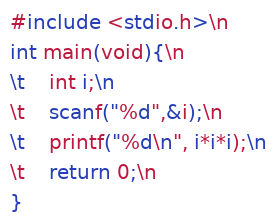
\includegraphics[width=.5\linewidth]{tokenized_data.png}
	\caption{Код, разделенный токенизатором}
	\label{fig:tokenized}
\end{figure}
\par На рисунке \ref{fig:tokenized} изображен текст, разбитый на токены, где токены отличаются цветом.
\par Изначально весь выбраный датасет был пропущен через модели Dino, CodeBert и UnixCoder, а полученные вектора сохранены в numpy файлы.
\par Так как для сравнения будет решаться задача классификации в качестве базового решения (baseline) был выбран наивный баесовский классификатор(Naive Bayes Classifier). Наивный байесовский классификатор был выбран поскольку он является классическим методом машинного обучения, широко применяемым для задач обработки текстовых данных. Во время предобработки, исходный текст был токензирован и в дальнейшем токены были трансформированны с помощью TF-IDF\@.
\subsubsection{Устойчивость представлений}
\par В рамках исследования проведено сравнение устойчивости векторных представлений, сгенерированных различными моделями, к синтаксическим вариациям исходного кода. Для этого были созданы модифицированные версии исходного кода, включающие добавление комментариев, добавление функци и намеренное допущение ошибок. Каждая версия кода была преобразована в векторное представление, после чего выполнено сравнение полученных векторов с исходным представлением при помощи метрики косинусного расстояния.
\par Этот эксперимент позволяет определить, насколько устойчивы векторные представления к незначительным изменениям в коде: хорошая модель должна выдавать близкие векторы для семантически эквивалентных программ, даже если их поверхностный синтаксис отличается. Например, если косинусное расстояние между представлениями остаётся малым при переименовании переменных, значит, модель захватывает смысл кода, а не его поверхностные особенности.
\begin{figure}[H]
    \centering
    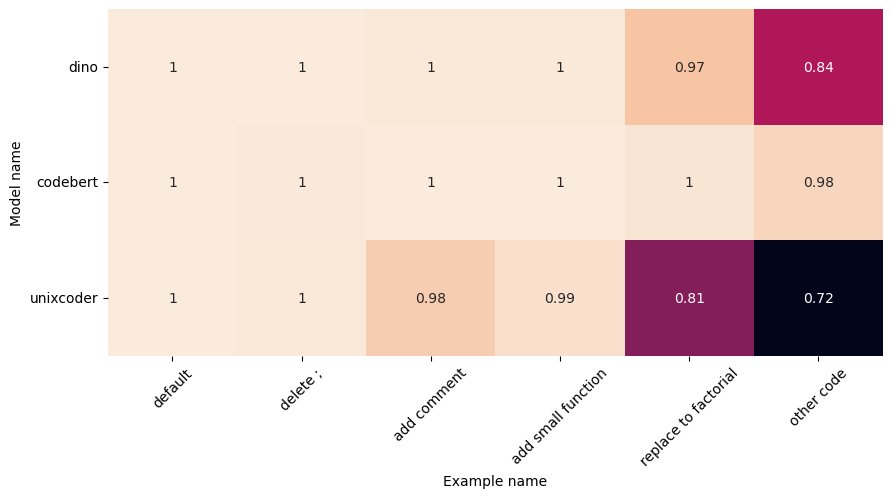
\includegraphics[width=0.8\textwidth]{robustness.png}
    \caption{Косинусное расстояние между default и другими версиями}
    \label{fig:robustness}
\end{figure}
\par Описание версий:
\begin{itemize}
    \item default - программа для вычисления $i$ числа последовательности Фибоначчи
    \item delete ; - код из которого были удалены все символы завершения
    \item add comment - добавлен однострочный комментарий
    \item add small function - добавленна функция суммирующая 2 переменные типа int
    \item replace to factorial - тело функции вычисления $i$ числа последовательности заменено на вычисление факториала
    \item other code - изначальное решение полностью изменнено и новое решение рисуте в консоли пирамидку из символов "*"
\end{itemize}
\par Проведенный анализ(\ref{fig:robustness}) выявил существенные различия в реакции исследуемых моделей на синтаксические изменения исходного кода:

\begin{itemize}
    \item Модель UniXcoder продемонстрировала наибольшую чувствительность к модификациям кода, реагируя на все значимые изменения включая добавление коментариев и небольших функций. Высокая чувствительность свидетельствует о способности модели улавливать тонкие семантические различия.

    \item Модель CodeBERT показала наименьшую реакцию на внесенные изменения, сохраняя близкие векторные представления даже при существенных модификациях кода. Это может указывать либо на чрезмерную обобщающую способность модели, либо на недостаточную чувствительность к локальным синтаксическим изменениям.

    \item Модель Dino заняла промежуточное положение, продемонстрировав сбалансированную реакцию: она надежно фиксировала значительные структурные изменения исходного кода, но при этом не проявляла избыточной чувствительности к незначительным синтаксическим вариациям.
\end{itemize}

\par Полученные результаты позволяют сделать вывод о том, что модель UniXcoder наиболее чуствительна, тогда как CodeBERT почти не реагирует на изменения. Модель Dino представляет собой компромиссный вариант, сочетающий разумную чувствительность к значимым изменениям с устойчивостью к несущественным модификациям.
\subsubsection{Визуализация токенных представлений через цветовое пространство}
\par Метод визуализации токенных представлений через цветовое представление позволяет интерпретировать семантические свойства текста через цветовую проекцию векторных представлений. Модель выдает похожие цвета семантически схожим токенам. Каждая из моделей обработала по 48 прмиеров решений, полученные представления для каждого из токенов в дальнейшем с помощью процесса снижения размерности t-SNE\cite{tsne} представления были ужаты до 3х мерных. Полученные вектора были нормализованны и использованны как цвет, для отображения токенов.

\begin{figure}[H]
	\centering
	\begin{subfigure}{.32\textwidth}
		\centering
		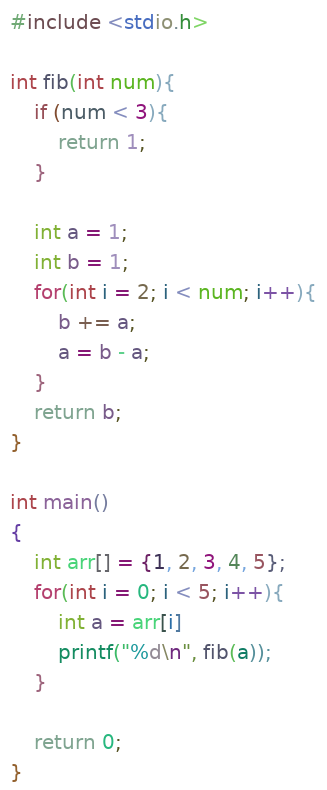
\includegraphics[width=.9\linewidth]{multicolor_texdino_48.png}
		\caption{DINO}
	\end{subfigure}
	\hfill
	\begin{subfigure}{.32\textwidth}
		\centering
		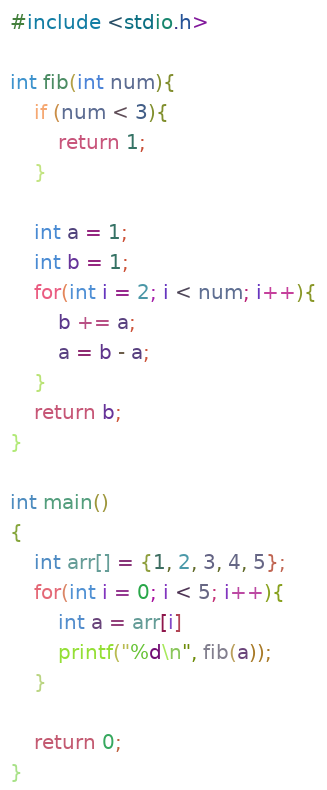
\includegraphics[width=.9\linewidth]{multicolor_texcodebert_48.png}
		\caption{CodeBERT}
	\end{subfigure}
	\hfill
	\begin{subfigure}{.32\textwidth}
		\centering
		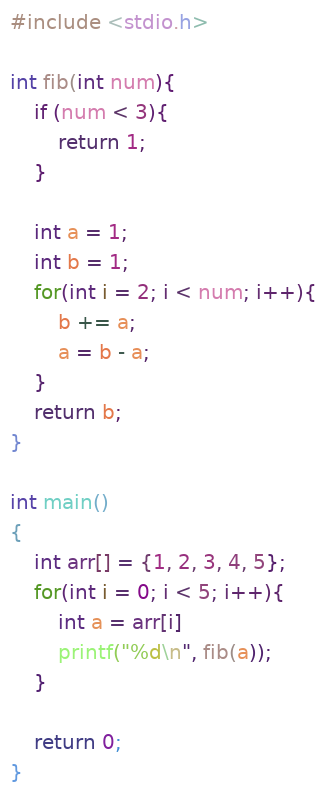
\includegraphics[width=.9\linewidth]{multicolor_texunixcoder_48.png}
		\caption{UnixCoder}
	\end{subfigure}
	\vspace{1cm}
\end{figure}
\par На основании представленных изображений можно сделать вывод, что модель Dino выделяет ключевые слова (такие как int, for, printf), при этом каждому ключевому слову назначается цвет, который не является заранее фиксированным (например, цвет может варьироваться в зависимости от того, определяет ли int локальную или глобальную переменную). Кроме того, в отличие от моделей CodeBert и UnixCoder, модель Dino присваивает различным переменным и константам разные цвета, что является важным отличием.
\subsubsection{Классификация номера задания}
\par Было выбрано 48 заданий из набора данных от IBM в которых больше всего принятых решений. Размер тренировочного набора - 65059. Размер тестового набора - 16265. После этого было решено использовать KNN классификатор и MLP классификатор предсказания номера задачи.
\par Для KNN был выставлен параметр - 10 ближайших соседей.
\par MLP имело 11 слоев, с функциями активации ReLU.
\begin{table}[H]
	\centering
	\begin{tabular}{|c|c||c|c|c|c|}\hline
		                        & BaseLine            &     & Dino & CodeBert & UnixCoder \\ \hline
		\multirow{2}{*}{Acc,\%} & \multirow{2}{*}{76} & KNN & 80      & 80       & 89        \\\cline{3-6}
		                        &                     & MLP & 85      & 81       & 95        \\\hline
	\end{tabular}
	\caption{Точность в процентах решения задачи определения номера задания}
\end{table}
\par Точность решения при помощи Dino значительно выше чем у baseline. Не уступает решению модели использующей представления модели CodeBert. Но в тоже время хуже, чем более сложная модель UnixCoder.
\subsubsection{Классификация статуса задачи}
\par Из прошлого набора данных было выбрано одно задание в котором было больше всего примеров. В качестве целевой переменной было выбрано булевое значение, которое отображает является ли задача принятой.
\par Размер тренировочного набора - 7838, из них 44\% приняты. Размер тестового набора - 1960, из них 44\% приняты.
\begin{table}[H]
	\centering
	\begin{tabular}{|c|c||c|c|c|c|}\hline
		                        & BaseLine            &     & Dino & CodeBert & UnixCoder \\ \hline
		\multirow{2}{*}{Acc,\%} & \multirow{2}{*}{72} & KNN & 72      & 72       & 73        \\\cline{3-6}
		                        &                     & MLP & 77      & 79       & 85        \\\hline
	\end{tabular}
	\caption{Точность в процентах решения задачи определения статуса решения}
\end{table}
\par Точность решений при помощи Dino значительно выше чем у baseline. В некоторых случаях уступает решению модели использующей представления модели CodeBert. И в тоже время хуже, чем более сложная модель UnixCoder. % #TODO Задача списывания
\end{document}